\section{The Hash-and-Resubmit Pattern}

In the Ethereum blockchain, the notion of Turing-complete smart contracts was
introduced. In order to prevent accidental of adversarial denial-of-service
phenomena such as infinite loops of code, contract invocations are bounded by
an amount of gas units(ref). Gas consumption determines the cost a user has to
pay in Ether(ref) to perform a function call, and constitutes one of the main
performance criteria of smart contracts. Towards the goal of implementing
gas-efficient smart contracts several patterns have been proposed.

\noindent \textbf{The Pattern.} We introduce a novel design pattern for
Solidity smart contracts that results into massive gas optimization. This
technique, which we term \emph{hash-and-resubmit}, is based on observing public
data of the blockchain in order to leverage \emph{off-chain} operations. By
utilizing this technique, the performance of the smart contract is improved
considerably since computations are performed locally by the user, and
gas-heavy storage variables are discarded.

The critical observation we make is that large structures, i.e. arrays, that
are sent to smart contracts and remain immutable, can be eliminated. This is
due to the fact that in the body of the Ethereum block, information regarding
transactions is stored. Nodes have access to this information which include the
signatures and input arguments of function invocations. Hence, a node can
access the information of a transaction by reading the blockchain instead of
invoking contract functions. This type of off-chain access can be applied by
any node.

\begin{figure}[h]
    \begin{center}
        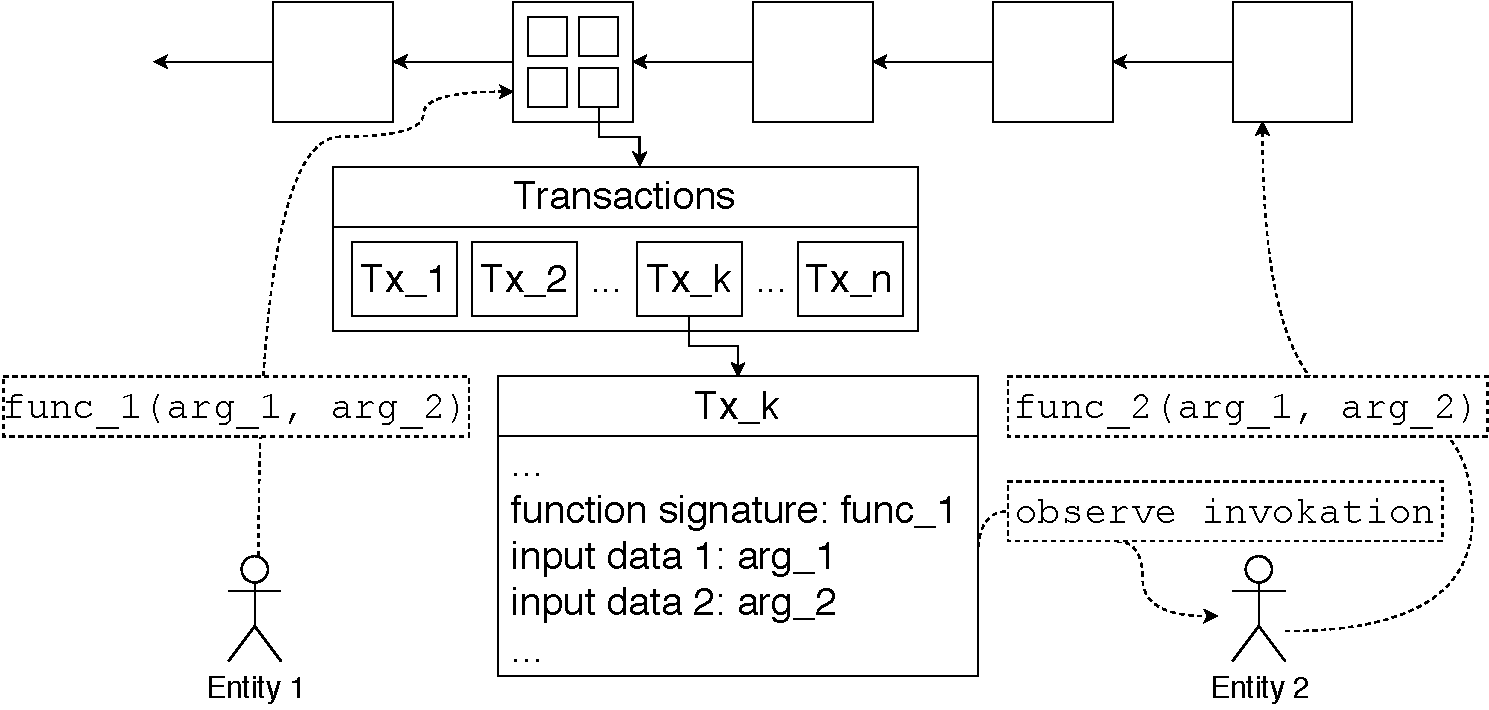
\includegraphics[width=1\columnwidth]{figures/observer-tx.pdf}
    \end{center}
    \caption{Entity 1 makes a function call with arguments arg1 and arg2.
    Entity 2 reads the content of transactions in the block and retrieves the
    input data. Entity 2 can use this data to make a different invocation.}
    \label{fig:observe-tx}
\end{figure}

\begin{algorithm}
    \label{alg.compare-storage}
    \caption{\textsf{Compare} N-sized arrays using storage}
    \begin{algorithmic}[1]
        \Function{\sf Submit}{$array$}
            \State $best\_array \gets array$
            \Comment{array saved in storage}
            \State $holder \gets msg.sender$
            \State\Return{true}
        \EndFunction
    \vskip8pt
    \end{algorithmic}

    \begin{algorithmic}[1]
        \Function{\sf Contest}{$new\_array$}
        \If{!compare($new\_array$)}
            \State\Return{false}
        \EndIf
        \State $holder \gets msg.sender$
        \State\Return{true}
    \EndFunction
    \vskip8pt
    \end{algorithmic}

    \begin{algorithmic}[1]
        \Function{\sf compare}{$new\_array$}
            \For{$i$ in $best\_array$.length}
            \If{$new\_array$[$i$] $\leq$ $best\_array$[$i$]}
                    \State\Return{false}
                \EndIf
            \EndFor
            \State\Return{true}
        \EndFunction
        \vskip8pt
    \end{algorithmic}
\end{algorithm}

\begin{algorithm}
    \label{alg.compare-memory}
    \caption{\textsf{Compare} N-sized arrays using hash-and-resubmit pattern}
    \begin{algorithmic}[1]
        \Function{\sf Submit}{$array[N]$}
        \State $hash \gets sha256(array)$
            \Comment{hash saved in storage}
            \State $holder \gets msg.sender$
            \State\Return{true}
        \EndFunction
    \vskip8pt
    \end{algorithmic}

    \begin{algorithmic}[1]
    \Function{\sf Contest}{$existing\_array$, $new\_array$}
    \If{hash256($existing\_array$) $\neq$ $hash$}
        \State\Return{false}
        \Comment{Invalid $original\_array$}
    \EndIf

    \If{!compare($original\_array$, $new\_array$)}
        \State\Return{false}
    \EndIf
    \State $holder \gets msg.sender$
    \State\Return{true}
    \EndFunction
    \vskip8pt
    \end{algorithmic}

    \begin{algorithmic}[1]
        \Function{\sf compare}{$array_1$, $array_2$}
            \For{$i$ in $array_1$.length}
                \If{$array_1$[$i$] $\leq$ $array_2$[$i$]}
                    \State\Return{false}
                \EndIf
            \EndFor
            \State\Return{true}
        \EndFunction
        \vskip8pt
    \end{algorithmic}
\end{algorithm}


As an example, we demonstrate a smart contract that implements a game between
two players $P1$, $P2$, in which the player with the most valuable array wins.
The contract consists of two phases: (a) Submit phase and (b) Contest phase.

\noindent \textbf{Submit
phase:} $P1$ submits an N-sized array, $array_1$ and becomes the
$holder$ of the contract.

\noindent \textbf{Contest phase:} $P2$ submits $array_2$. If $array_2$ $>$
$array_1$, then the holder of the contract is changed.

In this example, $array_1$ $>$ $array_2$ is true if $array_1$[$i$] $>$
$array_2$[$i$] is true for every $i$ $\in$ $array_1$.length. However, the
hash-and-resubmit pattern is agnostic to the implementation of the operator.

The rationale is to demand from $P2$ to provide two arrays to the contract
during contest phase: (a) $existing\_{array}$, which is a copy of the
originally submitted array by $P1$, and (b) $new\_array$, which is the
contesting array. The challenge here, is twofold:

\begin{enumerate}

    \item Availability: $P2$ must be able to retrieve a valid copy of
        $existing\_array$, without the need of accessing on-chain data.

    \item Reliability: We must prevent $P2$ from dispatching a malformed
        $existing\_array$ which differs from the originally submitted.

\end{enumerate}

As its name suggests, \emph{hash-and-resubmit} technique is performed in two
phases to face these challenges: the \emph{hash} phase, which addresses
\emph{reliability}, and the \emph{resubmit} phase which addresses
\emph{availability}.

\noindent

\textbf{Addressing Availability:} During submit-phase, $P1$ makes a call to the
function \texttt{submitEventProof}. This transaction, which consists of (a) the
function call and (b) the corresponding data, is added to a block by a miner.
As a blockchain transaction, the data of the function call are public to the
network. Due to blockchain's transparency, $P2$ can retrieve $array_1$ without
the need of accessing contract data. Note that this process is done off-chain.
$E_{cont}$ does not have to interact with the client.

\noindent

\textbf{Addressing Reliability:} We prevent an adversary from altering
$array_1$ by storing the hash of $array_1$ in contract's state during submit
phase and then verifying that $P2$ did not alter the original array by
verifying that the hash of claimed $array_1$ matches the hash of the original
submitted. We calculate the digest by invoking the pre-compiled \texttt{sha256}
hash function of Solidity:
\[\texttt{digest = sha256(abi.encodePacked(array))}\] The size of the digest of
a hash is 32 bytes. To persist such a small value in contract's memory only
adds a constant, negligible cost overhead to our implementation. This low-cost
technique allows us to provide vastly improved performance compared to the
previous work as we will show in the following subsections.

\noindent
\textbf{Benchmarks.} We demonstrate the implementation of the above game storage in
Algorithm~\ref{alg.compare-storage} and the hash-and-resubmit version in
Algorithm~\ref{alg.compare-memory}. The gas consumption of the two algorithms
is displayed in Figure~\ref{fig:har-example}.

\begin{figure}[h!]
\begin{center}
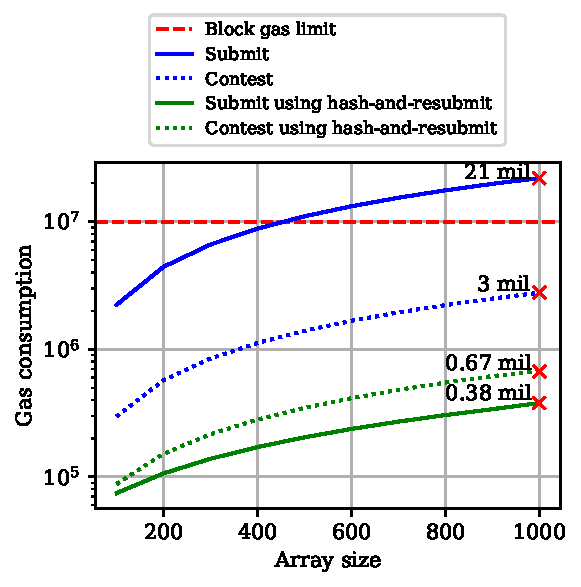
\includegraphics[width=1 \columnwidth]{figures/har-example.pdf}
\end{center}
\caption{Gas-cost reduction using the \emph{hash-and-resubmit} pattern. By
avoiding gas-heavy storage operations, the cost of function invocations is
decreased significantly by 93-95\%.}
\label{fig:har-example}
\end{figure}

We observe that, by using the hash-and-resubmit, the gas consumption of the
smart contracts is decreased by 93-95\%. This significantly affects the
applicability of the contract. Note that, the storage implementation exceeds the
Ethereum block gas limit\footnote{As of July 2020, the Ethereum block gas limit
is 10,000,000 gas units} for arrays of size 500 and above, contrary to the
hash-and-resubmit-optimized version, which consumes roughly 1/10th of the block
gas limit for arrays of 1000 elements.

\noindent \textbf{Enabling NIPoPoWs.} We now present how the
\emph{hash-and-resubmit} pattern can used in the context of the NIPoPoW
superlight client. Similar to our example game, the NIPoPoW verifier adheres to
submit-contest-phase schema and the inputs of the functions are arrays that are
processed on-chain. In \emph{submit-phase}, a \emph{proof} is submitted, and it
can be contested by another user in \emph{contest-phase}. The user that
initiates the contest, needs to monitor the traffic of the smart contract. This
is a logical assumption as mentioned in the NIPoPoW paper. The input of
\texttt{submit} function includes the \emph{proof} that indicates the
occurrence of an \emph{event} in the source chain and the input of
\texttt{contest} function includes the \emph{contesting proof}. A successful
challenge of the \emph{existing proof} is realized if the \emph{contesting
proof} has better score. The process of score evaluation is irrelevant to the
pattern and remains unchained.

In previous work~\cite{gglou}, NIPoPoW strings are stored on-chain during
submit-phase, and are processed during contest-phase. This operation is
performed by utilizing storage, which considerably limits the applicability of
the contract. In Algorithm~\ref{} we show how hash-and-resubmit pattern can be
embedded in the NIPoPoW client.

\newcommand{\genesis}{\textsf{G}}

\begin{algorithm}
    \label{alg:har-nipopow}
    \caption{The \textsf{NIPoPoW} client using hash-and-resubmit pattern}
    \begin{algorithmic}[1]

    \Contract{crosschain}
    \State $\textsf{events} \gets \bot;$ $\genesis \gets \bot$
    \Function{\sf initialize}{$\genesis_{remote}$}
        \State \genesis $\gets \genesis_{remote}$
    \EndFunction
    \Function{\sf submit}{$\pis$, $e$}
        \State \textsf{require}($\pis$[0] = $\genesis$)
        \State \textsf{require}($\textsf{events$[e]$} = \bot$)
        \State \textsf{require}($\textsf{valid-interlink}(\pi)$)
        \State \textsf{DAG} $\gets$ \textsf{DAG} $\cup$ $\pis$
        \State \textsf{events$[e]$.hash} $\gets$ \textsf{H}($\pis$)
        \Comment{enable pattern}
        \State \textsf{ancestors} $\gets$ \textsf{find-ancestors()}
        \State \textsf{events$[e]$.pred} $\gets$
            \textsf{evaluate-predicate}(\textsf{ancestors}, e)
        \State \textsf{ancestors} $=$ $\bot$
    \EndFunction
    \Function{\sf contest}{$\pisa$, $\pic$, $e$}
        \Comment{provide proofs}
        \State \textsf{require}(\textsf{events$[e]$.hash} $=$ \textsf{H}($\pisa$))
        \Comment{verify $\pisa$}
        \State \textsf{require}($\pic$[0] = $\genesis$)
        \State \textsf{require}(\textsf{events}$[e]$ $\ne$ $\bot$)
        \State \textsf{require}(\textsf{valid-interlink}($\pi_{cont}$))
        \State $lca$ = \textsf{find-lca}($\pisa$, $\pic$)
        \State \textsf{require}(\textsf{score}($\pic[:lca]$)
            $>$ \textsf{score}($\pisa[:lca]$))
        \State \textsf{DAG} $\gets$ \textsf{DAG} $\cup$ $\pic$
        \State \textsf{ancestors} $\gets$ \textsf{find-ancestors}(\textsf{DAG})
        \State \textsf{events$[e]$.pred} $\gets$
            \textsf{evaluate-predicate}(\textsf{ancestors}, $e$)
        \State \textsf{ancestors} $=$ $\bot$
    \EndFunction
    \EndContract
    \vskip8pt
    \end{algorithmic}
\end{algorithm}



% In previous work, storage was needed to persist submitted proofs and perform
% contests. In this subsection we show our novel approach to securely verify
% proofs without the utilization of persistent storage. We term this technique
% \emph{hash-and-resubmit}.
%
% The rationale is to demand from $E_{cont}$ to provide two proofs to the
% contract during contest phase: (a) $\pi_{exist}$, which is a copy of the
% originally submitted proof $\pi_{orig}$, and (b) $\pi_{cont}$, which is the
% contesting proof. The challenge here, is twofold:
%
% \begin{enumerate}
%
%     \item Availability: $E_{cont}$ must be able to retrieve a valid copy of $\pi_{orig}$,
%         $\pi_{exist}$ without the need of accessing on-chain data.
%
%     \item Reliability: We must prevent $E_{cont}$ from dispatching
%         $\tilde\pi_{exist}$ which differs from $\pi_{orig}$.
%
% \end{enumerate}
%
% As its name suggests, \emph{hash-and-resubmit} technique is performed in two
% phases to face this challenge: the \emph{hash} phase which addresses
% \emph{reliability}, and the \emph{resubmit} phase which addresses
% \emph{availability}.
%
% The corresponding changes are displayed in
% Algorithms~\ref{algorithm:submit_hash_and_resubmit}
%
% \paragraph{Addressing Availability:}
%
% During submit-phase, $E_{subm}$ makes a call to the function
% \texttt{submitEventProof}. This transaction, which consists of (a) the function
% call and (b) the corresponding data, is added to a block by a miner. As a
% blockchain transaction, the data of the function call are public to the
% network. Due to blockchain's transparency, $E_{cont}$ can retrieve
% $\pi_{orig}$ without the need of accessing contract data. This data space is
% called \emph{calldata}, and we make use of it to fetch $\pi_{exist}$, which is
% an exact copy of $\pi_{orig}$, originally submitted by $E_{subm}$. Note that
% this process is done off-chain. $E_{cont}$ does not have to interact with the
% client.
%
% \paragraph{Addressing Reliability:}
%
% We prevent an adversary from altering $\pi_{exist}$ by storing the hash of
% $\pi_{orig}$ in contract's state during submit phase and then verifying that
% $\pi_{exist}$ has the same hash. The operation of hashing the proof and storing
% the digest is cheap as shown in figure~\ref{figure:hash_proof_gas}. We
% calculate the digest by invoking the pre-compiled \texttt{sha256} hash function
% of Solidity:
%
% \[\texttt{digest = sha256(abi.encodePacked(proof))}\] The size of the digest of
% a hash is 32 bytes. To persist such a small value in contract's memory only
% adds a constant, negligible cost overhead to our implementation. This low-cost
% technique allows us to provide vastly improved performance compared to the
% previous work as we will show in the following subsections.
%
% \begin{algorithm}
    \caption{Contract State}
    \label{algo:hash_and_resubmit_data}
    \KwData{
      \texttt{Block} $genesis_{s}$,
      \texttt{\texttt{Bytes32} $digest^{\pi}$},
      \texttt{\texttt{Proof} $\pi_{s}$},
      \texttt{hashmap} $DAG_{s}$,
      \texttt{bool} $predicateExists_{s}$ \\
    }
\end{algorithm}

\begin{algorithm}
    \caption{Submit Event Proof}
    \label{algo:hash_and_resubmit_submit}
    \KwIn{\\
        \texttt{Proof} $\pi$, \\
        \texttt{Predicate} $predicate$
    }
    require $\pi[0]$ = $genesis_{s}$ \\
    require($predicateExists_{s}$ $=$ $false$) \\
    require($validInterlink(\pi$))\\
    $DAG_{s}$ $\leftarrow$ $DAG_{s}$ $\cup$ $\pi$\\
    $digest^{\pi}$ $\leftarrow$ sha256($\pi$) \\
    $ancestors_{s}$ $\leftarrow$ $findAncestors(DAG_{s}$)\\
    $predicateExists_{s}$ $\leftarrow$ $evaluatePredicate(ancestors_{s}$,
    $predicate$)\\
    delete $ancestors_{s}$\\
\end{algorithm}

\vspace{0.1cm}

\begin{algorithm}
    \caption{Submit Contest Proof}
    \label{algo:hash_and_resubmit_contest}
    \KwIn{\\
        \texttt{Proof} $\pi$, \texttt{Proof} $\tilde\pi$, \texttt{Predicate} $predicate$
    }
    require $\tilde\pi[0]$ = $genesis_{s}$ \\
    require($predicateExists_{s}$ = $true$) \\
    require(sha256($\pi$) = $digest^{\pi}$) \\
    $lca$ $\leftarrow$ findLca($\pi$, $\tilde\pi$) \\
    require($score(\tilde\pi[lca:])$ $>$ $score(\pi_{s}[lca:])$) \\
    require($score(\tilde\pi[lca:])$ $>$ $score(\pi[lca:])$) \\
    $DAG_{s}$ $\leftarrow$ $DAG_{s}$ $\cup$ $\tilde\pi$\\
    $ancestors_{s}$ $\leftarrow$ $findAncestors(DAG_{s})$\\
    $predicateExists_{s}$ $\leftarrow$ $evaluatePredicate(ancestors_{s}, predicate)$\\
    delete $ancestors_{s}$\\
\end{algorithm}


% \begin{figure}
\centering
\begin{tikzpicture}
    \begin{axis}[
        y tick label style={/pgf/number format/.cd,%
          set thousands separator={,},
          fixed},
        legend pos=north west,
        scaled y ticks = false,
        grid=major,
        xlabel={Proof size},
        ylabel={Gas consumption}]
    \addplot table [col sep=comma] {data/hash_proof_gas.csv};
    \legend{sha256 gas cost};
\end{axis}
\end{tikzpicture}
\caption{Gas consumption for hashing proofs and storing digest}
\label{figure:hash_proof_gas}
\end{figure}


